\chapter{Artificial Neural Networks}

Artificial neural networks are what makes the extension from traditional machine learning models into deep learning methods.

Classification tasks // regression tasks // computer vision and more...

\section{The Architecture of Neural Networks} %-------------SECTION

%---Pathway to Architecture file---
\subfile{Architecture}  

%\subsection{Gradient Descent}

%\subsubsection{Simulation in R}

%\subsection{Backpropagation}

%\subsubsection{Simulation in R}

\subsection{More Optimization Algorithms}

Aside from Gradient Descent.

Describe Stochastic Gradient Descent in subtle detail.

Make mention of other optimization algorithms (Adam, Adagrad, RMSprop), with only a brief description of them.  Only make mention of the ones to be used in Keras during practical examples in the next section.

\section{Types of Neural Networks} %-------------SECTION
The previous section described a \textbf{Multi-Layer Perceptron} network.  This section is devoted to other network types and their most practical uses. 

Obviously not all types will be covered, but here are a few.  

%\subsection{Multi-Layer Perceptron}
%Keras Model: "sequential"
%This ws described above

\subsection{Convolutional Neural Networks}
Unstructured image data

Convolution operation // Notation // Architecture and diagram

A Convolutional Neural Network (CNN) is a neural network that uses the convolution operation in at least one of its layers \cite{?}.

Convolution operation continuous
$$
C(t) = \int x(\tau)w(t - \tau)d\tau
$$
Convolution operation discrete
$$
C(t) = \sum_{\tau = -\infty}^\infty x(\tau)w(t - \tau)
$$
$x(t)$ is the \textbf{input} and $w(t-\tau)$ is known as the \textbf{kernel}. The shorthand operation for the convolution operation is denoted with an asterisk:
$$
(x * w)(t)
$$

Assumptions for CNN's \cite{Goodfellow-et-al-2016}

\begin{itemize}
  \tightlist
  \item
output is essentially a weighted average  
 \item
$w$ must be a valid probability distribution
 \item
$w$ is 0 for all negative arguments
 \item
values of kernel and input tensors are zero except for the finite set in which values are stored (i.e. size of image)
 \item
 - infinite summation over finite number of array elements
\end{itemize}


\subsubsection{Bird Call Spectrogram example from R}

\textit{(Make brief, include Keras code, stay on track that is is simply an illustration for CNN's)}

Labeled data on recorded bird calls converted into spectrograms of 251x251 pixels.

\begin{figure}[H]
\centering
    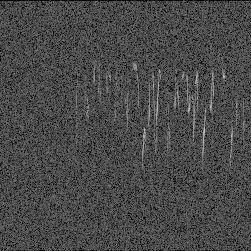
\includegraphics[width = .13\textwidth]{Figures/spectrogramsamps/Cardellina475957.png}
    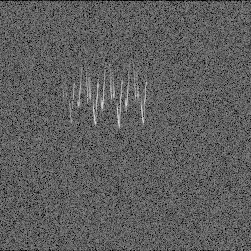
\includegraphics[width = .13\textwidth]{Figures/spectrogramsamps/Geothlypis13687.png}
    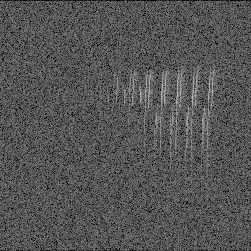
\includegraphics[width = .13\textwidth]{Figures/spectrogramsamps/Seiurus13640.png}
    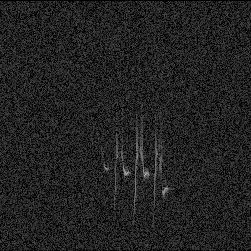
\includegraphics[width = .13\textwidth]{Figures/spectrogramsamps/Setophaga160916.png}
    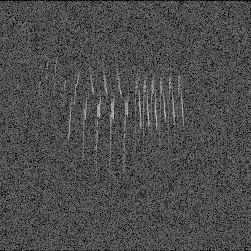
\includegraphics[width = .13\textwidth]{Figures/spectrogramsamps/Spinus192078.png}
    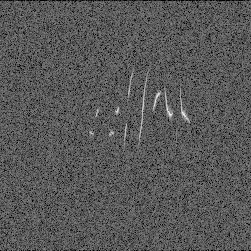
\includegraphics[width = .13\textwidth]{Figures/spectrogramsamps/Spizelloides45125.png}
    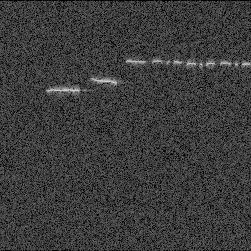
\includegraphics[width = .13\textwidth]{Figures/spectrogramsamps/Zonotrichia139053.png}
\end{figure}

Train the network to be able to identify that bird call based on spectrogram shape.

Use reference: \cite{kahl2017large}

Two-dimensional image $X$ with a two-dimensional kernel $W$
$$
C(i,j) = (X * W)(i,j) = \sum_m \sum_n X(m,n)W(i-m,j-n)
$$

$m$ and $n$ are the representative pixel locations in the relevant dimension, while $i$ and $j$ are the kernel locations, where the convolution is taking place.  The infinite summation is made possible by the fact that values are zero wherever the image is not present.



$$
Insert Example Here
$$

%---POTENTIALLY - make a pathway to the .tex file from RMarkdown ---\subfile{CNN_BCS} 


\subsection{Generative Adversarial Networks}
Unstructured image data

(Notation, no direct coding example)

Image generation to try and fool a "discriminator" network

\subsection{Recurrent Neural Networks}
Unstructured text data

(Notation, MAYBE time series coding example)

NLP/translation/text generation
Time series forecasting

\subsection{Long Short-Term Memory Network}
Unstructured text data

(Notation, no coding example)

\subsection{Convolutional Recurrent Networks}
Unstructured text data

(consider removing)

\section{Techniques to Improve Model Performance} %-------------SECTION

%---Pathway to performance file---
\subfile{Performance}